\documentclass{article}
\usepackage[utf8x]{inputenc}
\usepackage[russian]{babel}
\usepackage{amsmath}
\usepackage[a4paper, total={6in, 8in}]{geometry}
\usepackage{graphicx}
\graphicspath{{pictures/}}
\DeclareGraphicsExtensions{.pdf,.png,.jpg}
\author{Носков Роман, Пасютин Александр, Панчишин Даниил}
\title{Инструменты для оформления научных статей и презентаций (верстка текстового документа в Latex, оформление элементов текстового документа в \LaTeX, презентации в \LaTeX, работа с видео в \LaTeX-презентациях).}
\begin{document}
	\begin{center}
		\scriptsize{МИНИСТЕРСТВО НАУКИ И ВЫСШЕГО ОБРАЗОВАНИЯ РОССИЙСКОЙ ФЕДЕРАЦИИ
		
		Федеральное государственное бюджетное образовательное учреждение высшего образования
		
		«Кемеровский государственный университет»
		
		Институт фундаментальных наук
		
		Кафедра ЮНЕСКО по информационным вычислительным технологиям
	}
	\vspace{\baselineskip}
	
			\LARGE{\textbf{ОТЧЁТ}}
		
		\normalsize по учебной практике, технологической (проектно-технологической) практике
		
		проект «Инструменты для оформления научных статей и презентаций (верстка текстового документа в LaTeX, оформление элементов текстового документа в LaTeX, презентации в LaTeX, работа с видео в LaTeX-презентациях»
	\end{center}
\textbf{Выполнили:}

\noindent студенты направления подготовки 02.03.02 Фундаментальная информатика и информационные технологии, направленности (профиля) подготовки «Информатика и компьютерные науки»

\begin{flushright}
	
$\underset{\text{(ФИО)}}{\underline{\hspace{0.3\textwidth}}}$ $\underset{\text{(Оценка)}}{\underline{\hspace{0.1\textwidth}}}$ 
\vspace{\baselineskip}
		
$\underset{\text{(ФИО)}}{\underline{\hspace{0.3\textwidth}}}$ $\underset{\text{(Оценка)}}{\underline{\hspace{0.1\textwidth}}}$ 
\vspace{\baselineskip}

$\underset{\text{(ФИО)}}{\underline{\hspace{0.3\textwidth}}}$ $\underset{\text{(Оценка)}}{\underline{\hspace{0.1\textwidth}}}$ 
\end{flushright}
\newpage
\section*{Оглавление}
\LARGE{
1. Описание проекта \hspace{79mm} 3
\vspace{\baselineskip}

\noindent2. Состав группы участников проекта \hspace{35mm} 3
\vspace{\baselineskip}

Состав группы \hspace{87mm} 3
\vspace{\baselineskip}

Общие цели и задачи \hspace{72mm} 4
\vspace{\baselineskip}

Распределение по ролям \hspace{63mm} 4
\vspace{\baselineskip}

План-график работы \hspace{71mm} 5
\vspace{\baselineskip}

\noindent3. Ход работы \hspace{96mm} 8
\vspace{\baselineskip}

\noindent4. Литература} \hspace{93mm} 10
\newpage
\section{Описание проекта}
	\section*{Актуальность, теоретическая и практическая значимость:}
	
	
	\noindent\emph{Актуальность:}
	
	
	\noindent Нам, как студентам, необходимо знание редактора для оформления научных статей и презентаций.\\
	
	
	\noindent\emph{Теоретическая значимость:}
	
	
	\noindent Умение создания разверстанных научных статей и презентаций.\\
	
	
	\noindent\emph{Практическая значимость:}
	
	
	\noindent Наш проект позволит продемонстрировать группе возможности LaTeX’а.
	
\section{Состав группы участников проекта}
\subsection*{Состав группы}
\begin{tabular}{| l | l | l |p{5cm}|}
\hline
№ & ФИО & Логин на github.com \\
\hline
1. & Пасютин Александр Сергеевич & Antimagus \\
\hline
2. & Панчишин Даниил Игоревич & Donut42Russian \\
\hline
3. & Носков Роман Игоревич & DvojkaT \\
\hline
\end{tabular}
\subsection*{Общие цель и задачи}

\noindent\textbf{Цель:} научиться делать документы с высококачественной версткой текста, формул и других объектов

\subsection*{Задачи:}

\begin{itemize}
	\item Изучение инструментов и макропакетов ТеХ'а
	
	\item Получение навыков верстки текста в LaTeX’е
	
	\item Создание отчета по проекту в системе LaTeX
\end{itemize}
\subsection*{Распредение по ролям}
Панчишин Д.И. - Тимлид, создание тех задания, работа в LaTeX’е с мат. Формулами, псевдорисунки и графиками.

\vspace{\baselineskip}
Носков Р.И. - Работа в LaTeX’е с инструментами для верстки текста.

\vspace{\baselineskip}
Пасютин А.С. - Работа в LaTeX’е с инструментами для работы с презентациями, фотографиями.

\subsection*{План-график работы}
\begin{tabular}{|l|p{8,5cm}|}
	\hline
	18.02 & Распределение ролей, создание удаленного репозитория, составление календарного плана \\
	\hline
	4.03 & Изучение общего теоретического материала \\
	\hline
	18.03 & Начало работы над практической частью проекта \\
	\hline
	01.04 & Изучение отдельных аспектов \LaTeX’а, распределенных по ролям \\
	\hline
	15.04 & Создание презентации в \LaTeX, которая бы демонстрировала изученные навыки \\
	\hline
	29.04 & Создание отчета в \LaTeX, который бы демонстрировал изученные навыки
	\\
	\hline
	13.05 & Презентация результатов работы над проектом \\
	\hline
	27.05-31.05 & Защита проекта \\
	\hline
\end{tabular}

\subsection*{Что такое \TeX и \LaTeX}
\TeX — издательская система, созданная американским математиком и программистом Дональдом Кнутом (Donald E. Knuth). \TeX был разработан преследуя две основные цели: - позволить всем создавать качественные публикации с разумными для этого усилиями. \TeX знаменит своей чрезвычайной стабильностью, работой на различных операционных системах и практически полным отсутствием ошибок. Одна из главных причин по которой TeX выбирают для оформления научных работ заключается в том, что с его помощью можно достаточно легко вводить сложные формулы.

\vspace{\baselineskip}
\LaTeX — наиболее популярный набор макрорасширений (или макропакет) системы компьютерной вёрстки TeX, который облегчает набор сложных документов. Первая версия \LaTeX была написана в 1984 году Лесли Лампортом (Leslie Lamport) и с тех пор стала доминирующим способом подготовки \TeX публикаций. Важно заметить, что ни один из макропакетов для \TeX’а не может расширить \TeX’овских возможностей (всё, что можно сделать в LaTeX’е, можно сделать и в \TeX’е), но, благодаря различным упрощениям, использование макропакетов зачастую позволяет избежать весьма изощрённого программирования. Пакет позволяет автоматизировать многие задачи набора текста и подготовки статей, включая набор текста на нескольких языках, нумерацию разделов и формул, перекрёстные ссылки, размещение иллюстраций и таблиц на странице, ведение библиографии и др. Кроме базового набора существует множество пакетов расширения \LaTeX.

\subsection*{Используемые средства}

Для того чтобы писать \LaTeX на ПК под управлением Windows 10 нам понадобится загрузить и установить TexStudio(редактор для создания \TeX документов), а также MikTex(дистрибутив \TeX для Windows, необходимый для компиляции .tex файлов в .pdf).

\subsection*{Что представляет из себя \LaTeX документ}
Документ \LaTeX — это текстовый файл, содержащий специальные команды языка разметки. Сам документ делится на преамбулу и тело. Преамбула содержит информацию про класс документа, использованные пакеты макросов, определения макросов, автора, дату создания документа и другую информацию. Тело документа содержит собственно текст документа и команды разметки
	\section*{Цели и задачи:}
	
	
	\emph{Цель данной работы:} научиться делать документы с высококачественной версткой текста, формул и других объектов.\\
	
	
	\noindent\emph{Задачи:} изучение инструментов и макропакетов ТеХ'а, получение навыков верстки текста в ЛаТеХ'е, создание отчета по проекту в системе ЛаТеХ.
	
	
	\section*{Конечный результат:}
	Презентация и отчет о \LaTeX, созданные в \LaTeX.
	
	\section*{Ход работы}
	\subsection*{3.03 – 18.03:}
	
	Изучили особенности форматирования текста в системе LaTeX (русификация, шрифты, стили, разделы, интервалы, переносы)
	
	Изучили набор математических формул (строчные и выключные формулы, дроби, скобки, стандартные функции, символы, диакратические знаки и буквы других алфавитов)
	
	Создание презентаций (знакомство с пакетом Beamer, темы оформления, создание титульного слайда, оглавление презентации, поочередное появление объектов, выделение информации при помощи блоков и т.д.)
	
	\subsection*{18.03-15.04:}
	
	Создали в PowerPoint шаблон презентации, словарь команд \LaTeX для изменения шрифтов, заготовки отчета и презентации в \LaTeX
	
	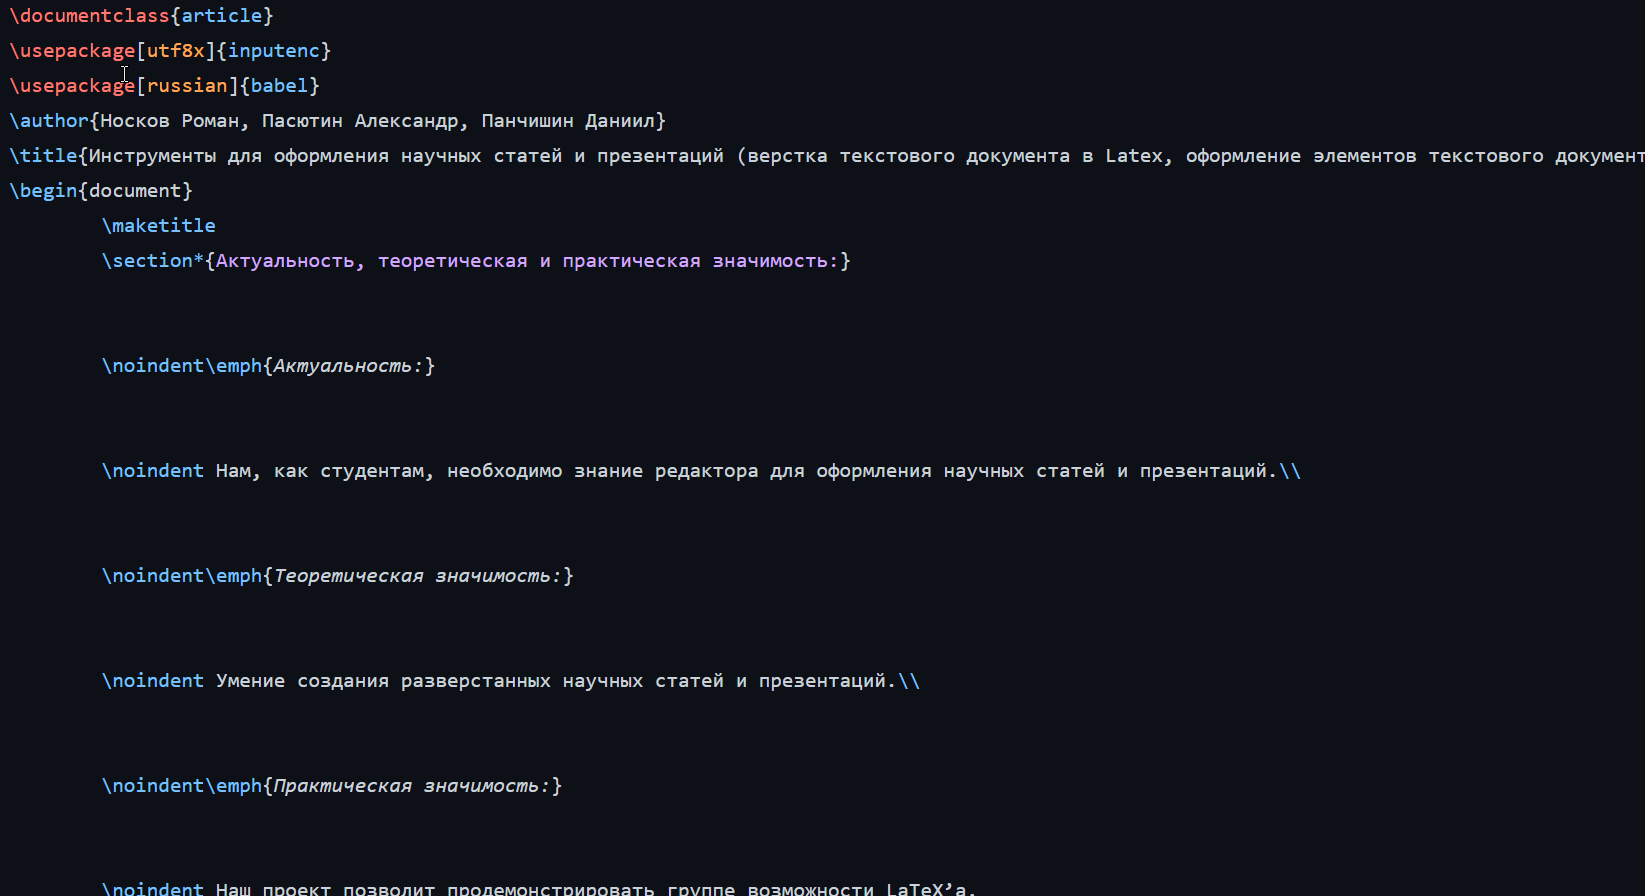
\includegraphics{1}
	
	
	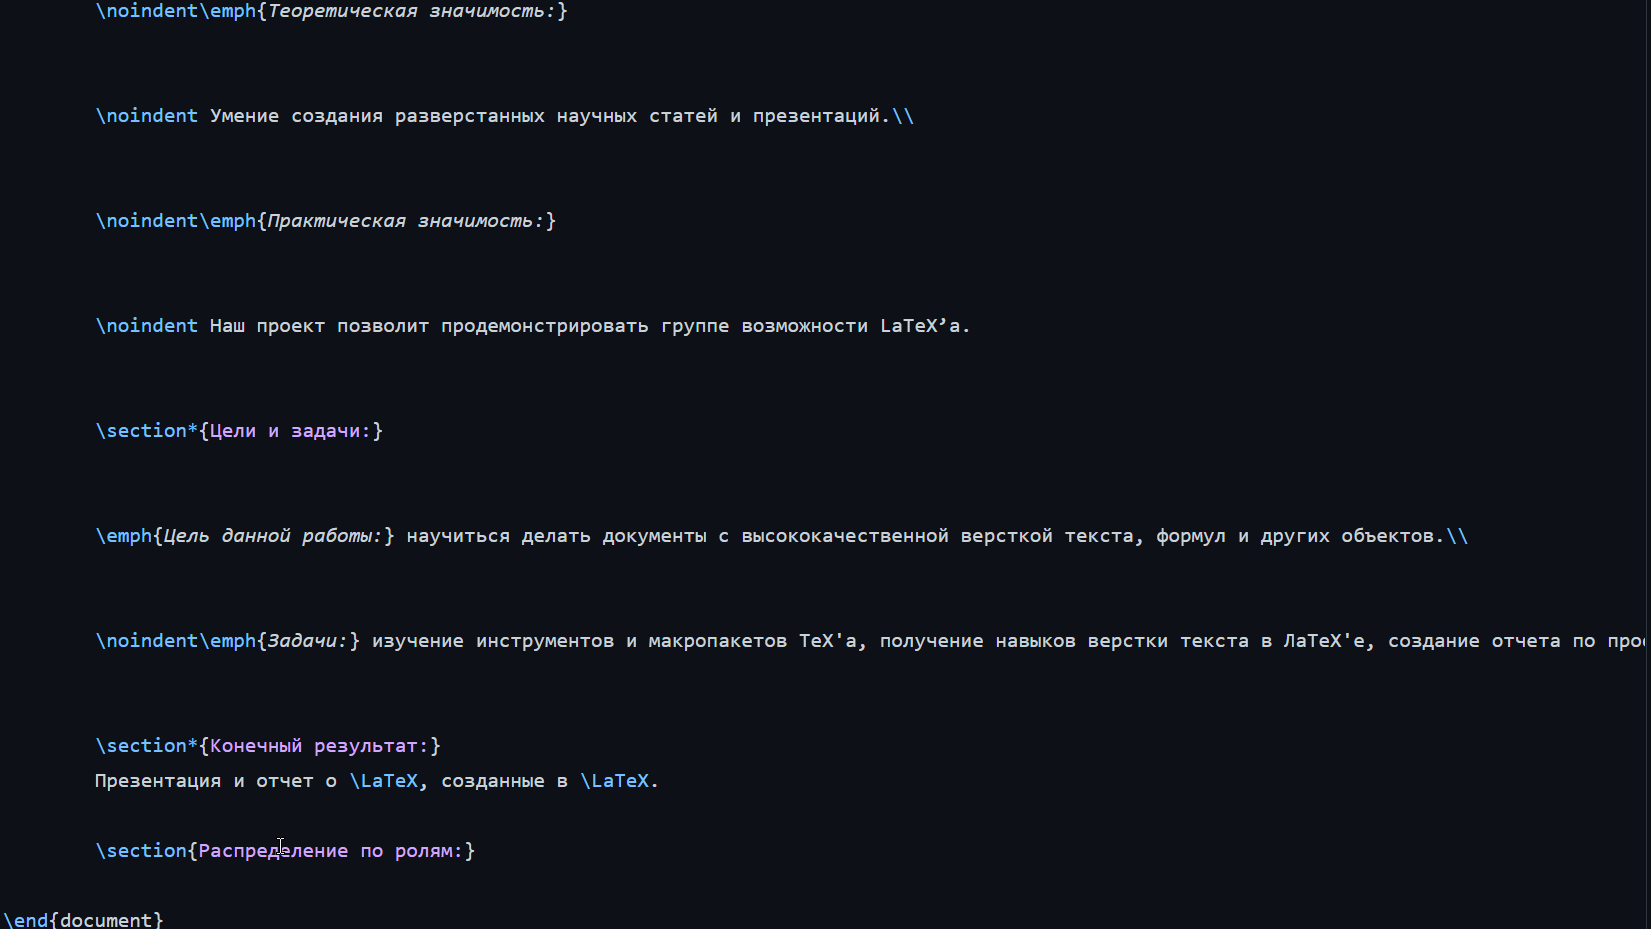
\includegraphics{2}
	
	
	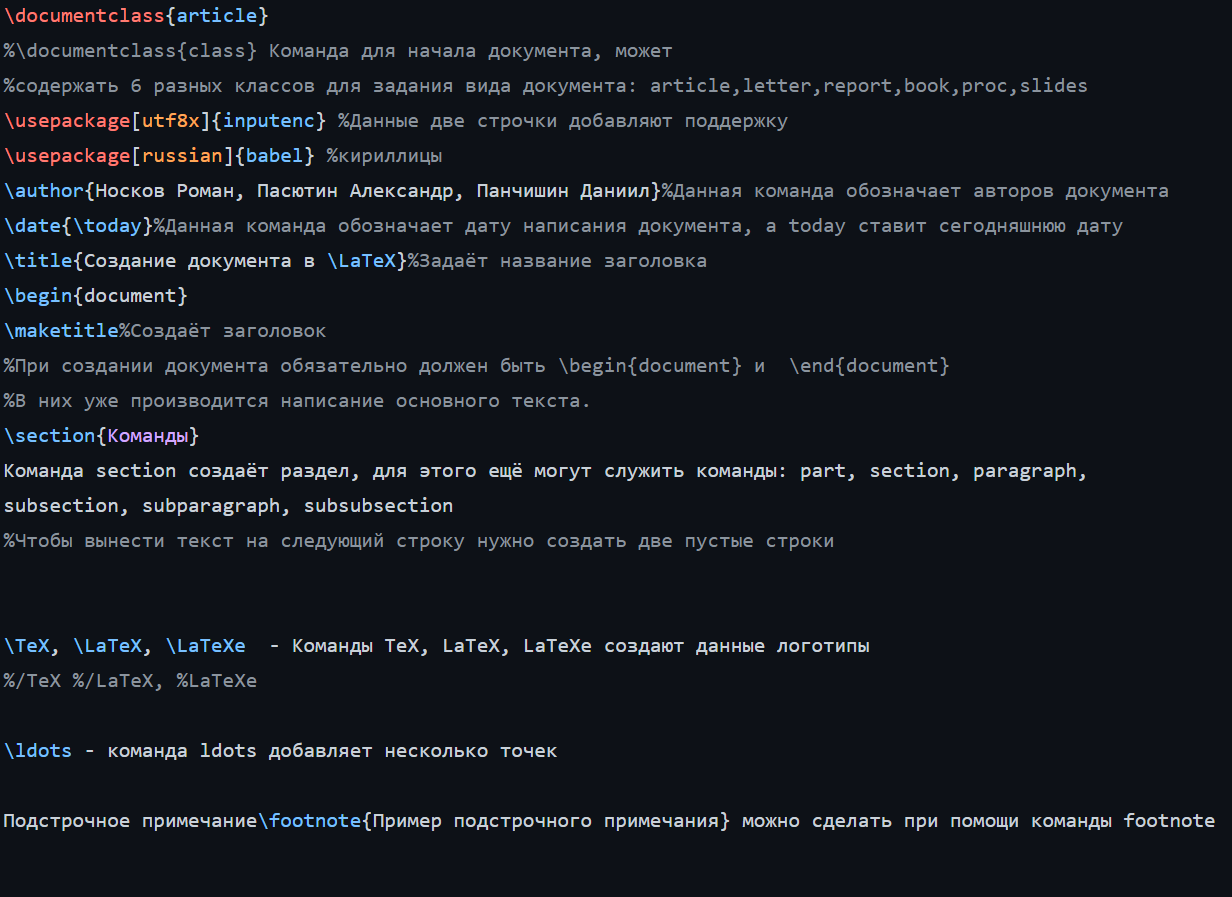
\includegraphics{3}
	
	
	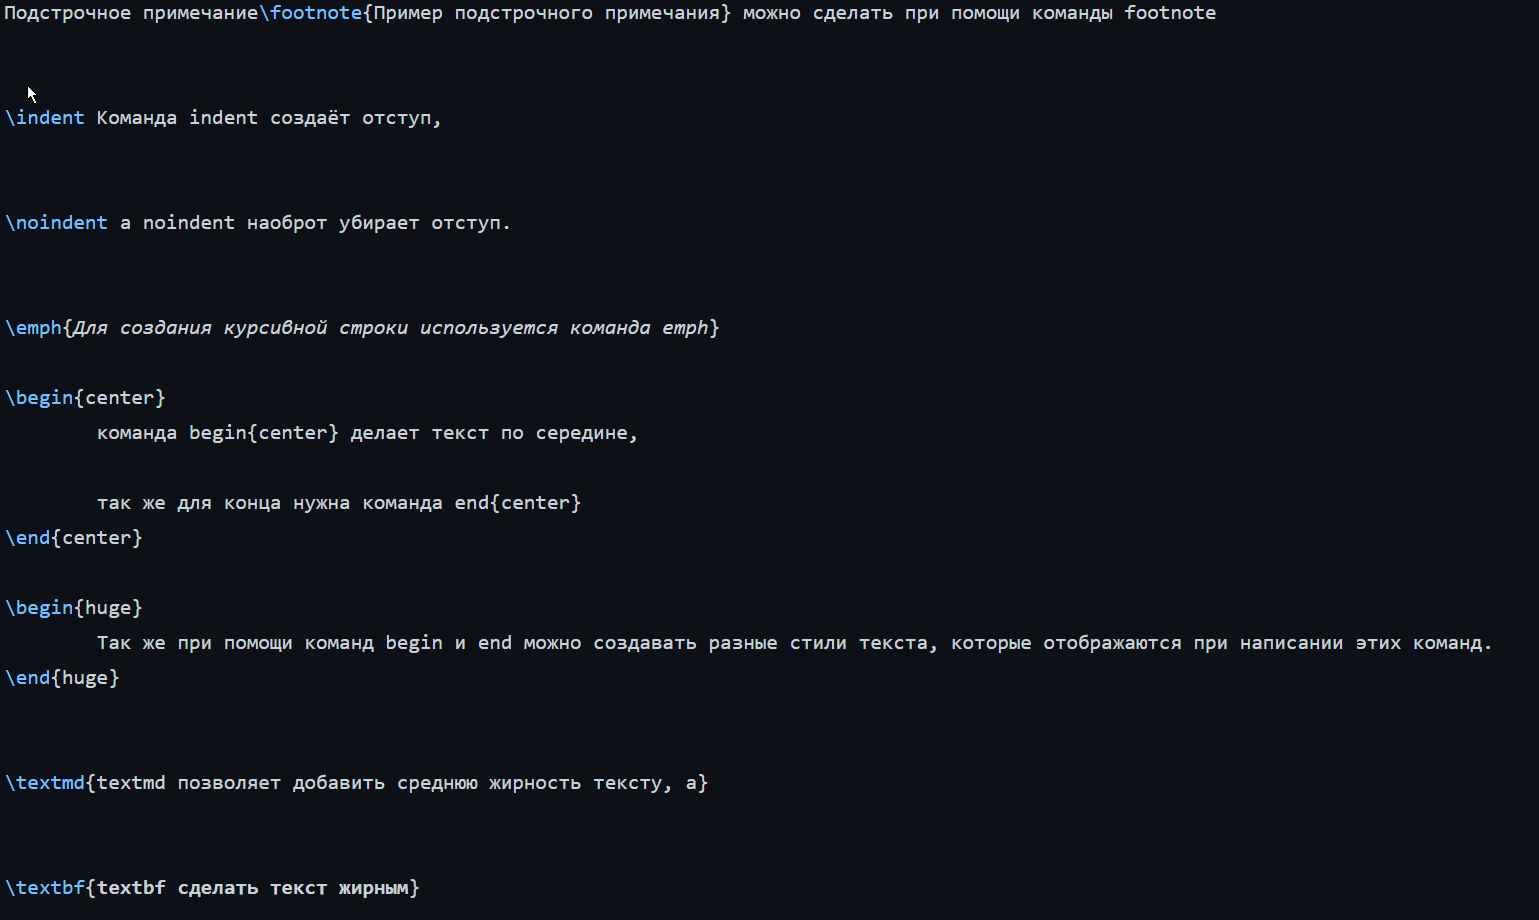
\includegraphics{4}
	
	
	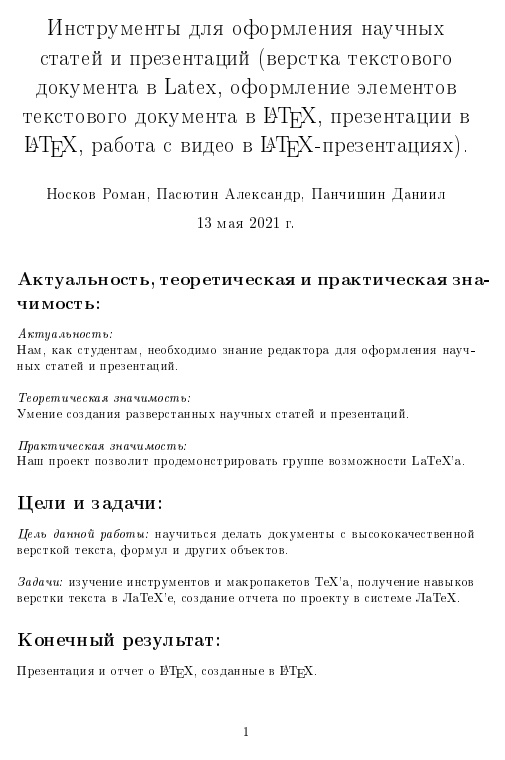
\includegraphics{5}
	
	
	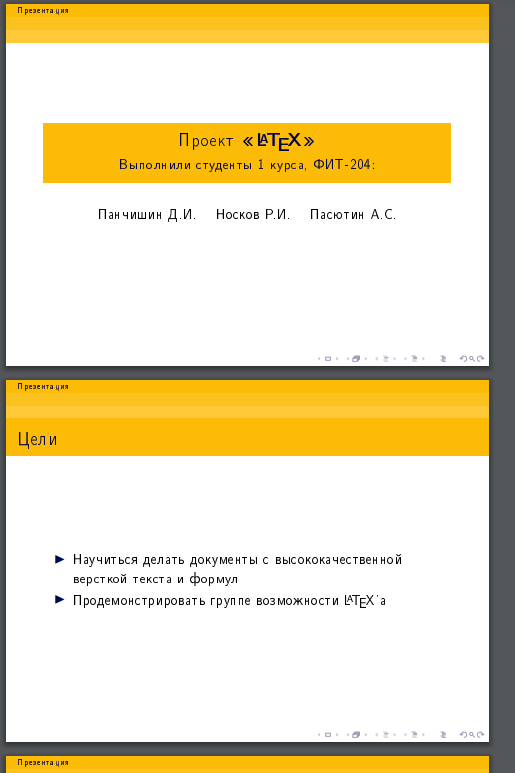
\includegraphics{6}
	
	
	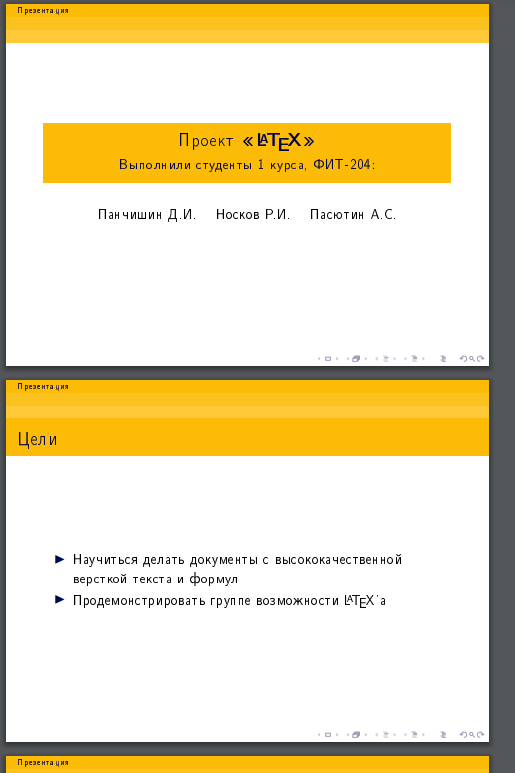
\includegraphics{7}
	
	
	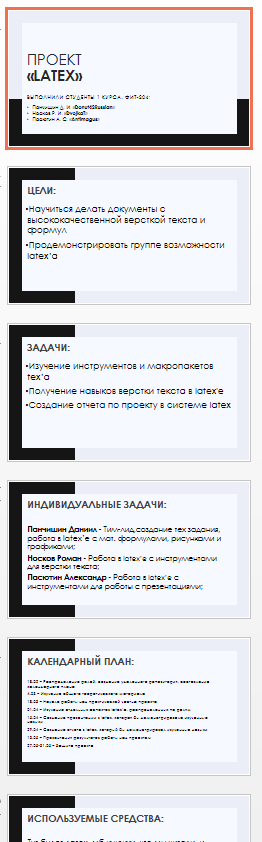
\includegraphics{8}
	
	
	
	\subsection*{15.04-13.05}
	
	Частично изучили класс для создания презентаций Beamer, работу с overlay’ами, рисунками, ссылками, кнопками, видео и листингом кода. Также были изучены ввод матриц, графиков и псевдорисунков. В области верстки текста было изучено создание таблиц.
	
	Были обновлены презентация и отчет. В презентацию добавлены примеры кода формул, графиков, псевдорисунков, их итогового отображения и кода отчета, также с итоговым отображением.
	
	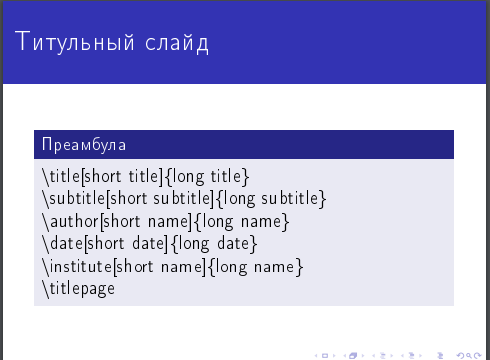
\includegraphics{9}
	
	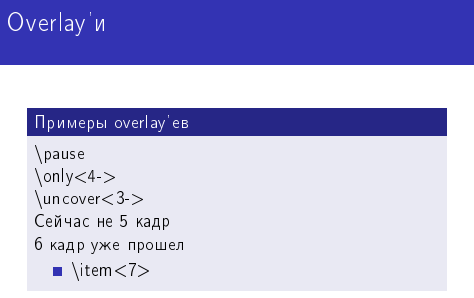
\includegraphics{10}
	
	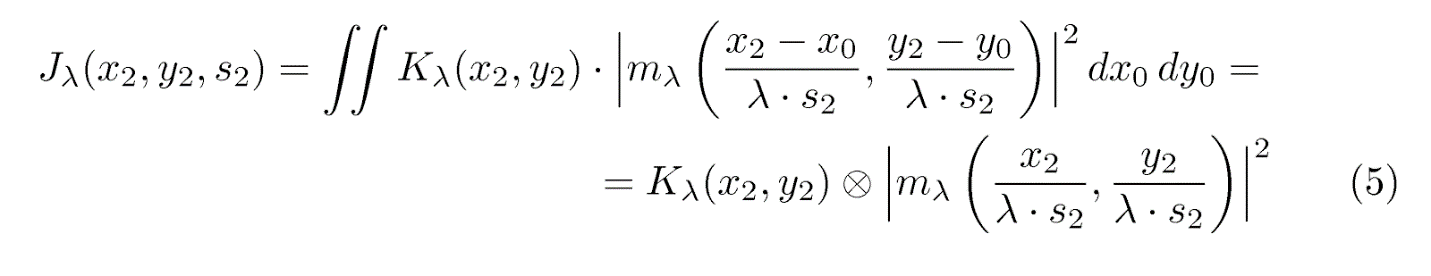
\includegraphics{11}
	
	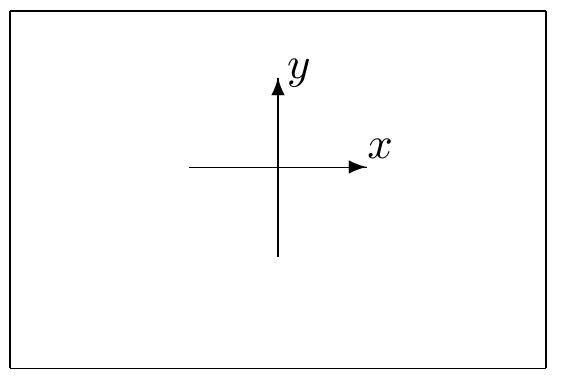
\includegraphics{12}
	
	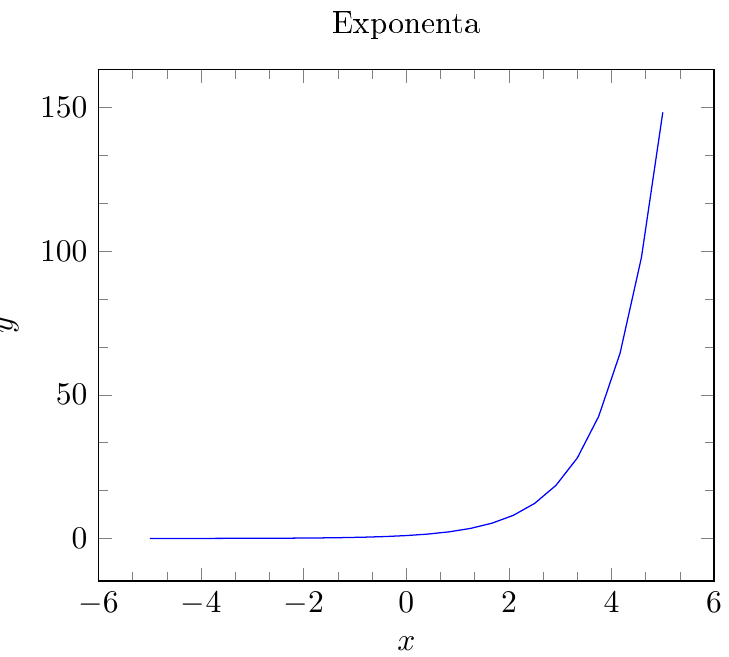
\includegraphics{13}
	
	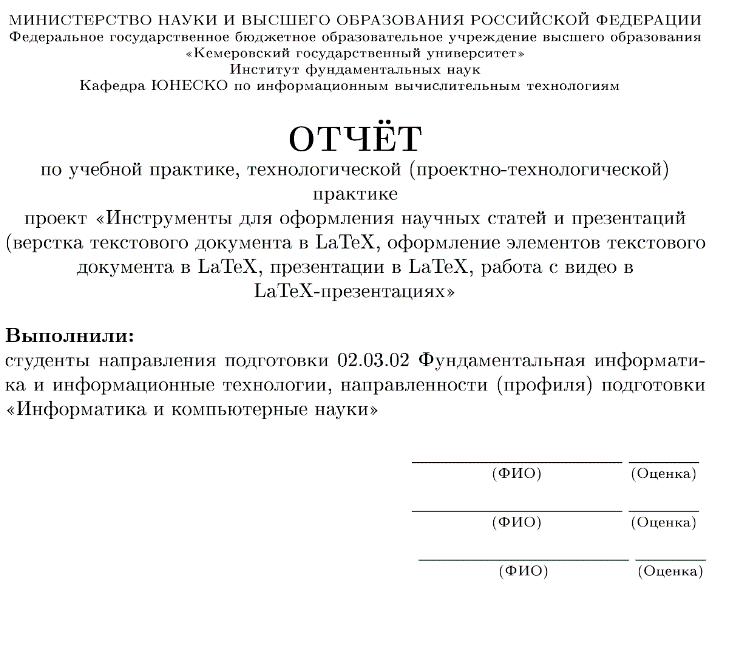
\includegraphics{14}
	
	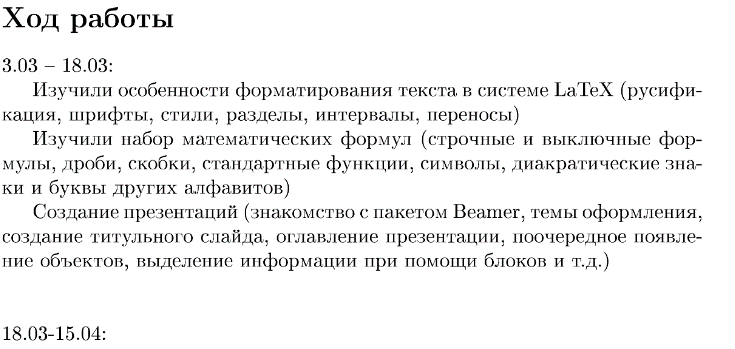
\includegraphics{15}
	
	\subsection*{13.05-27.05}
	
	Закончены и оформлены презентация и отчет. 
	
	\section{Литература}
	
	\begin{itemize}
		\item Львовский С. М. Набор и вёрстка в системе LaTeX. — М.: МЦНМО,
		 2006. — 448 с.
		 \item Котельников И. А., Чеботаев П. З. LaTeX по-русски. — СПб. : «Корона-Век», 2011. — 496 с.
		 \item Курс «Документы и презентации в LaTeX (Introduction to LaTeX)» на сайте coursera.org - https://www.coursera.org/learn/latex/home/welcome
	\end{itemize}
\end{document}